% Options for packages loaded elsewhere
\PassOptionsToPackage{unicode}{hyperref}
\PassOptionsToPackage{hyphens}{url}
%
\documentclass[
]{article}
\usepackage{amsmath,amssymb}
\usepackage{lmodern}
\usepackage{iftex}
\ifPDFTeX
  \usepackage[T1]{fontenc}
  \usepackage[utf8]{inputenc}
  \usepackage{textcomp} % provide euro and other symbols
\else % if luatex or xetex
  \usepackage{unicode-math}
  \defaultfontfeatures{Scale=MatchLowercase}
  \defaultfontfeatures[\rmfamily]{Ligatures=TeX,Scale=1}
\fi
% Use upquote if available, for straight quotes in verbatim environments
\IfFileExists{upquote.sty}{\usepackage{upquote}}{}
\IfFileExists{microtype.sty}{% use microtype if available
  \usepackage[]{microtype}
  \UseMicrotypeSet[protrusion]{basicmath} % disable protrusion for tt fonts
}{}
\makeatletter
\@ifundefined{KOMAClassName}{% if non-KOMA class
  \IfFileExists{parskip.sty}{%
    \usepackage{parskip}
  }{% else
    \setlength{\parindent}{0pt}
    \setlength{\parskip}{6pt plus 2pt minus 1pt}}
}{% if KOMA class
  \KOMAoptions{parskip=half}}
\makeatother
\usepackage{xcolor}
\usepackage[margin=1in]{geometry}
\usepackage{color}
\usepackage{fancyvrb}
\newcommand{\VerbBar}{|}
\newcommand{\VERB}{\Verb[commandchars=\\\{\}]}
\DefineVerbatimEnvironment{Highlighting}{Verbatim}{commandchars=\\\{\}}
% Add ',fontsize=\small' for more characters per line
\usepackage{framed}
\definecolor{shadecolor}{RGB}{248,248,248}
\newenvironment{Shaded}{\begin{snugshade}}{\end{snugshade}}
\newcommand{\AlertTok}[1]{\textcolor[rgb]{0.94,0.16,0.16}{#1}}
\newcommand{\AnnotationTok}[1]{\textcolor[rgb]{0.56,0.35,0.01}{\textbf{\textit{#1}}}}
\newcommand{\AttributeTok}[1]{\textcolor[rgb]{0.77,0.63,0.00}{#1}}
\newcommand{\BaseNTok}[1]{\textcolor[rgb]{0.00,0.00,0.81}{#1}}
\newcommand{\BuiltInTok}[1]{#1}
\newcommand{\CharTok}[1]{\textcolor[rgb]{0.31,0.60,0.02}{#1}}
\newcommand{\CommentTok}[1]{\textcolor[rgb]{0.56,0.35,0.01}{\textit{#1}}}
\newcommand{\CommentVarTok}[1]{\textcolor[rgb]{0.56,0.35,0.01}{\textbf{\textit{#1}}}}
\newcommand{\ConstantTok}[1]{\textcolor[rgb]{0.00,0.00,0.00}{#1}}
\newcommand{\ControlFlowTok}[1]{\textcolor[rgb]{0.13,0.29,0.53}{\textbf{#1}}}
\newcommand{\DataTypeTok}[1]{\textcolor[rgb]{0.13,0.29,0.53}{#1}}
\newcommand{\DecValTok}[1]{\textcolor[rgb]{0.00,0.00,0.81}{#1}}
\newcommand{\DocumentationTok}[1]{\textcolor[rgb]{0.56,0.35,0.01}{\textbf{\textit{#1}}}}
\newcommand{\ErrorTok}[1]{\textcolor[rgb]{0.64,0.00,0.00}{\textbf{#1}}}
\newcommand{\ExtensionTok}[1]{#1}
\newcommand{\FloatTok}[1]{\textcolor[rgb]{0.00,0.00,0.81}{#1}}
\newcommand{\FunctionTok}[1]{\textcolor[rgb]{0.00,0.00,0.00}{#1}}
\newcommand{\ImportTok}[1]{#1}
\newcommand{\InformationTok}[1]{\textcolor[rgb]{0.56,0.35,0.01}{\textbf{\textit{#1}}}}
\newcommand{\KeywordTok}[1]{\textcolor[rgb]{0.13,0.29,0.53}{\textbf{#1}}}
\newcommand{\NormalTok}[1]{#1}
\newcommand{\OperatorTok}[1]{\textcolor[rgb]{0.81,0.36,0.00}{\textbf{#1}}}
\newcommand{\OtherTok}[1]{\textcolor[rgb]{0.56,0.35,0.01}{#1}}
\newcommand{\PreprocessorTok}[1]{\textcolor[rgb]{0.56,0.35,0.01}{\textit{#1}}}
\newcommand{\RegionMarkerTok}[1]{#1}
\newcommand{\SpecialCharTok}[1]{\textcolor[rgb]{0.00,0.00,0.00}{#1}}
\newcommand{\SpecialStringTok}[1]{\textcolor[rgb]{0.31,0.60,0.02}{#1}}
\newcommand{\StringTok}[1]{\textcolor[rgb]{0.31,0.60,0.02}{#1}}
\newcommand{\VariableTok}[1]{\textcolor[rgb]{0.00,0.00,0.00}{#1}}
\newcommand{\VerbatimStringTok}[1]{\textcolor[rgb]{0.31,0.60,0.02}{#1}}
\newcommand{\WarningTok}[1]{\textcolor[rgb]{0.56,0.35,0.01}{\textbf{\textit{#1}}}}
\usepackage{graphicx}
\makeatletter
\def\maxwidth{\ifdim\Gin@nat@width>\linewidth\linewidth\else\Gin@nat@width\fi}
\def\maxheight{\ifdim\Gin@nat@height>\textheight\textheight\else\Gin@nat@height\fi}
\makeatother
% Scale images if necessary, so that they will not overflow the page
% margins by default, and it is still possible to overwrite the defaults
% using explicit options in \includegraphics[width, height, ...]{}
\setkeys{Gin}{width=\maxwidth,height=\maxheight,keepaspectratio}
% Set default figure placement to htbp
\makeatletter
\def\fps@figure{htbp}
\makeatother
\setlength{\emergencystretch}{3em} % prevent overfull lines
\providecommand{\tightlist}{%
  \setlength{\itemsep}{0pt}\setlength{\parskip}{0pt}}
\setcounter{secnumdepth}{-\maxdimen} % remove section numbering
\newlength{\cslhangindent}
\setlength{\cslhangindent}{1.5em}
\newlength{\csllabelwidth}
\setlength{\csllabelwidth}{3em}
\newlength{\cslentryspacingunit} % times entry-spacing
\setlength{\cslentryspacingunit}{\parskip}
\newenvironment{CSLReferences}[2] % #1 hanging-ident, #2 entry spacing
 {% don't indent paragraphs
  \setlength{\parindent}{0pt}
  % turn on hanging indent if param 1 is 1
  \ifodd #1
  \let\oldpar\par
  \def\par{\hangindent=\cslhangindent\oldpar}
  \fi
  % set entry spacing
  \setlength{\parskip}{#2\cslentryspacingunit}
 }%
 {}
\usepackage{calc}
\newcommand{\CSLBlock}[1]{#1\hfill\break}
\newcommand{\CSLLeftMargin}[1]{\parbox[t]{\csllabelwidth}{#1}}
\newcommand{\CSLRightInline}[1]{\parbox[t]{\linewidth - \csllabelwidth}{#1}\break}
\newcommand{\CSLIndent}[1]{\hspace{\cslhangindent}#1}

\usepackage{tcolorbox}

\definecolor{mybluebackground}{HTML}{e7f3fe}
\definecolor{mybluecolor}{HTML}{31708f}
\definecolor{myblueborder}{HTML}{bce8f1}
\definecolor{mybrownbackground}{HTML}{f9f0e4}
\definecolor{mybrowncolor}{HTML}{8a6d3b}
\definecolor{mybrownborder}{HTML}{faebcc}

\newtcolorbox{infobox}{
  colback=mybluebackground,
  colframe=myblueborder,
  coltext=mybluecolor,
  boxsep=3pt,
  boxrule=1pt,
  arc=4pt}

\newtcolorbox{warningbox}{
  colback=mybrownbackground,
  colframe=mybrownborder,
  coltext=mybrowncolor,
  boxsep=3pt,
  boxrule=1pt,
  arc=4pt}

\usepackage{amsmath}
\usepackage{booktabs}
\usepackage{float}
\usepackage{subcaption}
\usepackage{caption}
\floatplacement{figure}{H}
\usepackage{booktabs}
\usepackage{longtable}
\usepackage{array}
\usepackage{multirow}
\usepackage{wrapfig}
\usepackage{float}
\usepackage{colortbl}
\usepackage{pdflscape}
\usepackage{tabu}
\usepackage{threeparttable}
\usepackage{threeparttablex}
\usepackage[normalem]{ulem}
\usepackage{makecell}
\usepackage{xcolor}
\ifLuaTeX
  \usepackage{selnolig}  % disable illegal ligatures
\fi
\IfFileExists{bookmark.sty}{\usepackage{bookmark}}{\usepackage{hyperref}}
\IfFileExists{xurl.sty}{\usepackage{xurl}}{} % add URL line breaks if available
\urlstyle{same} % disable monospaced font for URLs
\hypersetup{
  pdftitle={Exploring the latitudinal gradient of utilised plants species richness and endemism},
  pdfauthor={Ian Ondo},
  hidelinks,
  pdfcreator={LaTeX via pandoc}}

\title{Exploring the latitudinal gradient of utilised plants species
richness and endemism}
\author{Ian Ondo}
\date{2023-07-24}

\begin{document}
\maketitle

{
\setcounter{tocdepth}{2}
\tableofcontents
}
\begin{warningbox}

\textbf{Package notes:}\\
We need to install the following set of R packages to successfully run
the codes in this vignette:

\begin{itemize}
\tightlist
\item
  \textbf{ComplexHeatmap} (Gu 2022)
\item
  \textbf{terra} (Hijmans 2023)
\item
  \textbf{mgcv} (S. N. Wood 2017)
\item
  \textbf{purrr} (Wickham and Henry 2023)
\item
  \textbf{circlize} (Gu et al. 2014)
\end{itemize}

\end{warningbox}

\hypertarget{introduction}{%
\section{Introduction}\label{introduction}}

In this vignette, we will investigate the variation in the latitudinal
gradient profiles of utilised species richness and endemism across
different plants uses (Pironon S. 2023) using Generalised Additive
Models (GAMs) (S. N. Wood 2011).\\
We need species richness/endemism maps of per use category and for all
uses confounded. If you do not have these maps yet, please have a look
at the vignette
\href{}{\textbf{\textcolor{black}{\underline{Mapping species distribution, richness and endemism}}}}.
We will demonstrate how to run the analyses with the species richness
maps, but the process is similar for the endemism.

\hypertarget{step-1-prepare-the-data-for-model-fitting}{%
\section{Step 1: Prepare the data for model
fitting}\label{step-1-prepare-the-data-for-model-fitting}}

Let's assume that we stored our species richness maps predictions (all
uses confounded and per uses) as Tagged Image Format (TIF) files in a
folder named ``\texttt{usefulplants\_species\_richness\_maps}'', then:

\begin{Shaded}
\begin{Highlighting}[]

\CommentTok{\# load all maps into R}
\NormalTok{all\_maps\_files }\OtherTok{\textless{}{-}} \FunctionTok{list.files}\NormalTok{(}\StringTok{"path/to/usefulplants\_species\_richness\_maps"}\NormalTok{,}
                             \AttributeTok{pattern=}\StringTok{"}\SpecialCharTok{\textbackslash{}\textbackslash{}}\StringTok{.tif$"}\NormalTok{, }\AttributeTok{full.names=}\ConstantTok{TRUE}\NormalTok{)}
\NormalTok{all\_maps\_rast }\OtherTok{\textless{}{-}}\NormalTok{ terra}\SpecialCharTok{::}\FunctionTok{rast}\NormalTok{(all\_maps\_files)}

\CommentTok{\# get the total species richness only}
\NormalTok{raster\_ref }\OtherTok{\textless{}{-}}\NormalTok{ all\_maps\_rast[[}\StringTok{"GlobalSR"}\NormalTok{]] }\CommentTok{\# change with the name of the "all uses" map}

\CommentTok{\# get the species richness per plants uses only}
\NormalTok{raster\_uses }\OtherTok{\textless{}{-}} \FunctionTok{subset}\NormalTok{(all\_maps\_rast, }\AttributeTok{subset=}\StringTok{"GlobalSR"}\NormalTok{, }\AttributeTok{negate=}\ConstantTok{TRUE}\NormalTok{)}

\CommentTok{\# vector of latitude values}
\NormalTok{ylat }\OtherTok{\textless{}{-}}\NormalTok{ terra}\SpecialCharTok{::}\FunctionTok{yFromRow}\NormalTok{(raster\_ref,}\AttributeTok{row=}\DecValTok{1}\SpecialCharTok{:}\FunctionTok{nrow}\NormalTok{(raster\_ref))}

\CommentTok{\# number of valid values by row}
\NormalTok{nna }\OtherTok{\textless{}{-}}\FunctionTok{apply}\NormalTok{(}\FunctionTok{as.matrix}\NormalTok{(raster\_ref[[}\DecValTok{1}\NormalTok{]],}\AttributeTok{wide=}\ConstantTok{TRUE}\NormalTok{),}\DecValTok{1}\NormalTok{,}\ControlFlowTok{function}\NormalTok{(x) }\FunctionTok{sum}\NormalTok{(}\SpecialCharTok{!}\FunctionTok{is.na}\NormalTok{(x)))}
\NormalTok{lat }\OtherTok{\textless{}{-}}\NormalTok{ base}\SpecialCharTok{::}\FunctionTok{rep}\NormalTok{(ylat, }\AttributeTok{times=}\NormalTok{nna)}

\CommentTok{\# get the valid cells per raster row}
\NormalTok{row\_valid\_cells }\OtherTok{\textless{}{-}} \FunctionTok{apply}\NormalTok{(}\FunctionTok{as.matrix}\NormalTok{(raster\_ref[[}\DecValTok{1}\NormalTok{]],}\AttributeTok{wide=}\ConstantTok{TRUE}\NormalTok{), }\DecValTok{1}\NormalTok{,}
                         \ControlFlowTok{function}\NormalTok{(x) }\FunctionTok{which}\NormalTok{(}\SpecialCharTok{!}\FunctionTok{is.na}\NormalTok{(x)))}
\end{Highlighting}
\end{Shaded}

\hypertarget{step-2-fit-generalised-additive-models}{%
\section{Step 2: Fit Generalised Additive
Models}\label{step-2-fit-generalised-additive-models}}

We are going to use the function \texttt{bam} from the \textbf{mgcv}
package to estimate our latitudinal gradient patterns. It provides
faster inference for large datasets.

\begin{Shaded}
\begin{Highlighting}[]

\NormalTok{to\_keep }\OtherTok{\textless{}{-}} \FunctionTok{complete.cases}\NormalTok{(all\_maps\_rast) }\CommentTok{\# keep track of valid rows}
\NormalTok{all\_maps\_rast}\SpecialCharTok{$}\NormalTok{lat }\OtherTok{\textless{}{-}}\NormalTok{ lat }\CommentTok{\# add the latitude vector}

\CommentTok{\# fit GAMs for each plants species richness distribution as a function of the latitude}
\NormalTok{my\_gam\_pred }\OtherTok{\textless{}{-}}\NormalTok{ all\_maps\_rast[to\_keep,] }\SpecialCharTok{\%\textgreater{}\%}
  \CommentTok{\# remove latitude as response variable}
\NormalTok{  dplyr}\SpecialCharTok{::}\FunctionTok{select}\NormalTok{(}\SpecialCharTok{{-}}\NormalTok{lat) }\SpecialCharTok{\%\textgreater{}\%} 
  \CommentTok{\# fit a GAM on with a penalised cublic regression spline as smoother for the latitude}
\NormalTok{  purrr}\SpecialCharTok{::}\FunctionTok{map}\NormalTok{(}\SpecialCharTok{\textasciitilde{}}\NormalTok{ mgcv}\SpecialCharTok{::}\FunctionTok{bam}\NormalTok{(.x }\SpecialCharTok{\textasciitilde{}} \FunctionTok{s}\NormalTok{(lat, }\AttributeTok{bs=}\StringTok{"cr"}\NormalTok{), }
                         \AttributeTok{family =} \StringTok{"Gamma"}\NormalTok{,}
                         \AttributeTok{data=}\NormalTok{all\_maps\_rast[to\_keep,],}
                         \AttributeTok{discrete=}\ConstantTok{TRUE}\NormalTok{)) }\SpecialCharTok{\%\textgreater{}\%}
  \CommentTok{\# predict for unique latitude values}
\NormalTok{  purrr}\SpecialCharTok{::}\FunctionTok{map}\NormalTok{(\textbackslash{}(mod) }\FunctionTok{predict}\NormalTok{(mod,}
                            \AttributeTok{newdata=}\FunctionTok{data.frame}\NormalTok{(}\AttributeTok{lat=}\FunctionTok{unique}\NormalTok{(lat)), }
                            \AttributeTok{type=}\StringTok{"response"}\NormalTok{)) }\SpecialCharTok{\%\textgreater{}\%}
\FunctionTok{do.call}\NormalTok{(cbind,.)}

\NormalTok{my\_gam\_pred}
\end{Highlighting}
\end{Shaded}

\hypertarget{step-3-prepare-the-data-for-the-heatmap-visualisation}{%
\section{Step 3: Prepare the data for the heatmap
visualisation}\label{step-3-prepare-the-data-for-the-heatmap-visualisation}}

We now have smoothed species richness predictions per latitude for each
plants uses and all uses at once. Next step is to compute differences
between each individual plant use categories and the ``all uses''
estimates taken as a baseline. In our example the ``all uses''
predictions (and maps) are called ``GlobalSR'', make sure to update the
following code to distinguish yours accordingly.

\begin{Shaded}
\begin{Highlighting}[]

\CommentTok{\# matrix of deviation of plants uses\textquotesingle{} species richness from the "all uses" baseline pattern}
\NormalTok{delta\_SR\_matrix\_scaled }\OtherTok{\textless{}{-}}\NormalTok{ my\_gam\_pred }\SpecialCharTok{\%\textgreater{}\%}
  \FunctionTok{as.data.frame}\NormalTok{() }\SpecialCharTok{\%\textgreater{}\%}
  \CommentTok{\# scaled the predictions to obtain proportions per latitudinal values}
\NormalTok{  dplyr}\SpecialCharTok{::}\FunctionTok{mutate\_all}\NormalTok{(}\SpecialCharTok{\textasciitilde{}}\NormalTok{ .}\SpecialCharTok{/}\FunctionTok{sum}\NormalTok{(.,}\AttributeTok{na.rm=}\ConstantTok{TRUE}\NormalTok{)) }\SpecialCharTok{\%\textgreater{}\%} 
  \CommentTok{\# calculate differences}
\NormalTok{  dplyr}\SpecialCharTok{::}\FunctionTok{mutate}\NormalTok{(dplyr}\SpecialCharTok{::}\FunctionTok{across}\NormalTok{(}\SpecialCharTok{{-}}\NormalTok{dplyr}\SpecialCharTok{::}\FunctionTok{starts\_with}\NormalTok{(}\StringTok{"Global"}\NormalTok{),}
                              \SpecialCharTok{\textasciitilde{}}\NormalTok{ . }\SpecialCharTok{{-}}\NormalTok{ GlobalSR, }\AttributeTok{.names =} \StringTok{"delta\{col\}"}\NormalTok{)) }\SpecialCharTok{\%\textgreater{}\%} 
\NormalTok{  dplyr}\SpecialCharTok{::}\FunctionTok{select}\NormalTok{(dplyr}\SpecialCharTok{::}\FunctionTok{starts\_with}\NormalTok{(}\StringTok{"delta"}\NormalTok{)) }\SpecialCharTok{\%\textgreater{}\%} \CommentTok{\# select plants use categories only}
\NormalTok{  dplyr}\SpecialCharTok{::}\FunctionTok{rename\_all}\NormalTok{(}\SpecialCharTok{\textasciitilde{}} \FunctionTok{gsub}\NormalTok{(}\StringTok{"delta|SR"}\NormalTok{,}\StringTok{""}\NormalTok{,.)) }\SpecialCharTok{\%\textgreater{}\%} \CommentTok{\# remove suffices}
  \FunctionTok{as.matrix}\NormalTok{()}

\CommentTok{\# retrieve the "all uses" (scaled) predictions only}
\NormalTok{my\_gam\_pred\_SR\_ref }\OtherTok{\textless{}{-}}\NormalTok{ my\_gam\_pred }\SpecialCharTok{\%\textgreater{}\%}
  \FunctionTok{as.data.frame}\NormalTok{() }\SpecialCharTok{\%\textgreater{}\%}
\NormalTok{  dplyr}\SpecialCharTok{::}\FunctionTok{mutate\_at}\NormalTok{(dplyr}\SpecialCharTok{::}\FunctionTok{vars}\NormalTok{(GlobalSR), }\SpecialCharTok{\textasciitilde{}}\NormalTok{ .}\SpecialCharTok{/}\FunctionTok{sum}\NormalTok{(.,}\AttributeTok{na.rm=}\ConstantTok{TRUE}\NormalTok{)) }\SpecialCharTok{\%\textgreater{}\%}
\NormalTok{  dplyr}\SpecialCharTok{::}\FunctionTok{pull}\NormalTok{(GlobalSR)}
\end{Highlighting}
\end{Shaded}

\hypertarget{step-4-create-a-heatmap-of-the-variation-of-the-species-richness-among-plants-uses-along-the-latitudinal-gradient}{%
\section{Step 4: Create a heatmap of the variation of the species
richness among plants uses along the latitudinal
gradient}\label{step-4-create-a-heatmap-of-the-variation-of-the-species-richness-among-plants-uses-along-the-latitudinal-gradient}}

We have a matrix of relative differences in species richness per
latitude between each plants use categories and all confounded uses. We
are going to use the package \textbf{Complexheatmap} to better visualise
these differences.

\begin{Shaded}
\begin{Highlighting}[]

\CommentTok{\# remove missing values and predictions in Antartica}
\NormalTok{to\_remove }\OtherTok{\textless{}{-}} \SpecialCharTok{!}\FunctionTok{complete.cases}\NormalTok{(delta\_SR\_matrix\_scaled) }\SpecialCharTok{|}\NormalTok{ (}\FunctionTok{unique}\NormalTok{(lat) }\SpecialCharTok{\textless{}} \SpecialCharTok{{-}}\DecValTok{50}\NormalTok{) }

\NormalTok{ylat }\OtherTok{\textless{}{-}}\NormalTok{ gam\_pred\_use\_sr}\SpecialCharTok{$}\NormalTok{Lat[}\SpecialCharTok{!}\NormalTok{to\_remove]}

\CommentTok{\# create a pre{-}heatmap to compute the dendogram}
\NormalTok{my.pre.heat.map }\OtherTok{\textless{}{-}}\NormalTok{ ComplexHeatmap}\SpecialCharTok{::}\FunctionTok{Heatmap}\NormalTok{(}
\NormalTok{  delta\_SR\_matrix\_scaled[}\SpecialCharTok{!}\NormalTok{to\_remove,]}
\NormalTok{)}

\NormalTok{ht }\OtherTok{\textless{}{-}}\NormalTok{ ComplexHeatmap}\SpecialCharTok{::}\FunctionTok{draw}\NormalTok{(my.pre.heat.map)}
\NormalTok{col\_order }\OtherTok{\textless{}{-}}\NormalTok{ ComplexHeatmap}\SpecialCharTok{::}\FunctionTok{column\_order}\NormalTok{(ht)}

\CommentTok{\# rotate the dendogram}
\NormalTok{column\_dendo }\OtherTok{=} \FunctionTok{as.dendrogram}\NormalTok{(ComplexHeatmap}\SpecialCharTok{::}\FunctionTok{column\_dend}\NormalTok{(ht))}

\CommentTok{\# to visualise}
\CommentTok{\# plot(column\_dendo \%\textgreater{}\%}
\CommentTok{\#        dendextend::set("labels\_colors")}
\CommentTok{\# )}

\CommentTok{\# optional: preferential ordering of categories}
\NormalTok{my.order }\OtherTok{\textless{}{-}} \FunctionTok{c}\NormalTok{(}\StringTok{"AnimalFood"}\NormalTok{,}\StringTok{"Materials"}\NormalTok{,}\StringTok{"Medicines"}\NormalTok{,}\StringTok{"GeneSources"}\NormalTok{,}
              \StringTok{"EnvironmentalUses"}\NormalTok{,}\StringTok{"HumanFood"}\NormalTok{,}\StringTok{"SocialUses"}\NormalTok{,}\StringTok{"Poisons"}\NormalTok{,}
              \StringTok{"InvertebrateFood"}\NormalTok{,}\StringTok{"Fuels"}\NormalTok{)}

\CommentTok{\#to visualise}
\CommentTok{\# plot(column\_dendo \%\textgreater{}\%}
\CommentTok{\#        dendextend::set("labels\_colors") \%\textgreater{}\%}
\CommentTok{\#        dendextend::rotate(my.order)}
\CommentTok{\# )}

\NormalTok{column\_dendogrm }\OtherTok{\textless{}{-}}\NormalTok{ column\_dendo }\SpecialCharTok{\%\textgreater{}\%}
\NormalTok{  dendextend}\SpecialCharTok{::}\FunctionTok{set}\NormalTok{(}\StringTok{"labels\_colors"}\NormalTok{) }\SpecialCharTok{\%\textgreater{}\%}
\NormalTok{  dendextend}\SpecialCharTok{::}\FunctionTok{rotate}\NormalTok{(col\_order)}

\NormalTok{new\_col\_order }\OtherTok{\textless{}{-}} \FunctionTok{labels}\NormalTok{(column\_dendogrm)}
\end{Highlighting}
\end{Shaded}

\hypertarget{define-top-annotations}{%
\subsection{Define top annotations}\label{define-top-annotations}}

\begin{Shaded}
\begin{Highlighting}[]

\CommentTok{\# optional font parameter}
\FunctionTok{windowsFonts}\NormalTok{(}\StringTok{"sans"} \OtherTok{=} \FunctionTok{windowsFont}\NormalTok{(}\StringTok{"sans"}\NormalTok{))}
\NormalTok{my\_font\_family}\OtherTok{=}\StringTok{"sans"}

\CommentTok{\# get the paths to useful plants icons}
\NormalTok{icons\_paths }\OtherTok{\textless{}{-}} \FunctionTok{list.files}\NormalTok{(}\FunctionTok{system.file}\NormalTok{(}\StringTok{"man/figures"}\NormalTok{,}\AttributeTok{package=}\StringTok{"UsefulPlants"}\NormalTok{),}
                          \AttributeTok{pattern=}\StringTok{"(Uses|Food|s)}\SpecialCharTok{\textbackslash{}\textbackslash{}}\StringTok{.png$"}\NormalTok{, }\AttributeTok{full.names=}\ConstantTok{TRUE}\NormalTok{)}

\NormalTok{anno\_joyplot\_list }\OtherTok{\textless{}{-}}\NormalTok{ my\_gam\_pred }\SpecialCharTok{\%\textgreater{}\%}
\NormalTok{  dplyr}\SpecialCharTok{::}\FunctionTok{select}\NormalTok{(}\SpecialCharTok{{-}}\NormalTok{GlobalSR,}\SpecialCharTok{{-}}\NormalTok{Lat) }\SpecialCharTok{\%\textgreater{}\%}
\NormalTok{  dplyr}\SpecialCharTok{::}\FunctionTok{mutate\_all}\NormalTok{(}\SpecialCharTok{\textasciitilde{}}\NormalTok{ .}\SpecialCharTok{/}\FunctionTok{sum}\NormalTok{(.,}\AttributeTok{na.rm=}\ConstantTok{TRUE}\NormalTok{)) }\SpecialCharTok{\%\textgreater{}\%}
\NormalTok{  dplyr}\SpecialCharTok{::}\FunctionTok{filter}\NormalTok{(}\SpecialCharTok{!}\NormalTok{to\_remove) }\SpecialCharTok{\%\textgreater{}\%}
\NormalTok{  purrr}\SpecialCharTok{::}\FunctionTok{map}\NormalTok{(}\SpecialCharTok{\textasciitilde{}} \FunctionTok{data.frame}\NormalTok{(}\AttributeTok{x=}\NormalTok{ylat,}\AttributeTok{y=}\NormalTok{.))}

\CommentTok{\# restricted vector of latitudes}
\NormalTok{ylat }\OtherTok{\textless{}{-}}\NormalTok{ my\_gam\_pred}\SpecialCharTok{$}\NormalTok{Lat[}\SpecialCharTok{!}\NormalTok{to\_remove]}

\CommentTok{\# top heatmap annotations}
\NormalTok{my.top.annotations }\OtherTok{\textless{}{-}}\NormalTok{ ComplexHeatmap}\SpecialCharTok{::}\FunctionTok{HeatmapAnnotation}\NormalTok{(}

  \StringTok{"Uses"} \OtherTok{=}\NormalTok{ ComplexHeatmap}\SpecialCharTok{::}\FunctionTok{anno\_image}\NormalTok{(icons\_paths,}
                                      \AttributeTok{height =}\NormalTok{ grid}\SpecialCharTok{::}\FunctionTok{unit}\NormalTok{(}\FloatTok{1.8}\NormalTok{, }\StringTok{"cm"}\NormalTok{),}
                                      \AttributeTok{width =}\NormalTok{ grid}\SpecialCharTok{::}\FunctionTok{unit}\NormalTok{(}\DecValTok{3}\NormalTok{, }\StringTok{"cm"}\NormalTok{),}
                                      \AttributeTok{border=}\ConstantTok{FALSE}\NormalTok{),}
  \StringTok{"Species richness}\SpecialCharTok{\textbackslash{}n}\StringTok{per use"} \OtherTok{=}\NormalTok{ ComplexHeatmap}\SpecialCharTok{::}\FunctionTok{anno\_joyplot}\NormalTok{(anno\_joyplot\_list,}
                            \AttributeTok{gp =}\NormalTok{ grid}\SpecialCharTok{::}\FunctionTok{gpar}\NormalTok{(}\AttributeTok{lwd=}\DecValTok{1}\NormalTok{, }\AttributeTok{col=}\StringTok{\textquotesingle{}black\textquotesingle{}}\NormalTok{,}
                                            \AttributeTok{fill=}\ConstantTok{NA}\NormalTok{,}
                                            \AttributeTok{transparency =} \FloatTok{0.25}\NormalTok{),}
                                  \AttributeTok{scale=}\FloatTok{0.6}\NormalTok{,}
                                \AttributeTok{width =}\NormalTok{ grid}\SpecialCharTok{::}\FunctionTok{unit}\NormalTok{(}\DecValTok{2}\NormalTok{, }\StringTok{"cm"}\NormalTok{),}
                                \AttributeTok{which=}\StringTok{"column"}\NormalTok{,}
                                \AttributeTok{axis\_param =} \FunctionTok{list}\NormalTok{(}
                                  \AttributeTok{side =} \StringTok{"right"}\NormalTok{,}
                                  \AttributeTok{at =} \FunctionTok{c}\NormalTok{(}\FloatTok{66.5}\NormalTok{, }\FloatTok{23.5}\NormalTok{, }\DecValTok{0}\NormalTok{, }\SpecialCharTok{{-}}\FloatTok{23.5}\NormalTok{),}
                                  \AttributeTok{gp =}\NormalTok{ grid}\SpecialCharTok{::}\FunctionTok{gpar}\NormalTok{(}\AttributeTok{fontface=}\FunctionTok{c}\NormalTok{(}\DecValTok{3}\NormalTok{,}\DecValTok{3}\NormalTok{,}\DecValTok{4}\NormalTok{,}\DecValTok{3}\NormalTok{),}
                                                  \AttributeTok{fontsize=}\DecValTok{14}\NormalTok{,}
                                                  \AttributeTok{fontfamily=}\NormalTok{my\_font\_family),}
                                  \AttributeTok{labels=}\FunctionTok{c}\NormalTok{(}\StringTok{"Arctic Circle"}\NormalTok{,}
                                           \StringTok{"Tropic of Cancer"}\NormalTok{,}
                                           \StringTok{"Equator"}\NormalTok{,}
                                           \StringTok{"Tropic of Capricorn"}\NormalTok{),}
                                  \AttributeTok{labels\_rot =} \DecValTok{0}\NormalTok{)}
\NormalTok{                            ),}
  \AttributeTok{annotation\_name\_gp =}\NormalTok{ grid}\SpecialCharTok{::}\FunctionTok{gpar}\NormalTok{(}\AttributeTok{fontfamily=}\NormalTok{my\_font\_family, }\AttributeTok{fontsize =} \DecValTok{20}\NormalTok{),}
  \AttributeTok{annotation\_name\_side =} \StringTok{"left"}\NormalTok{,}
  \AttributeTok{border=}\ConstantTok{TRUE}\NormalTok{,}
  \AttributeTok{show\_annotation\_name =} \FunctionTok{c}\NormalTok{(}\AttributeTok{Uses =} \ConstantTok{FALSE}\NormalTok{),}
  \AttributeTok{which=}\StringTok{\textquotesingle{}column\textquotesingle{}}
\NormalTok{)}
\end{Highlighting}
\end{Shaded}

\hypertarget{define-left-annotations}{%
\subsection{Define left annotations}\label{define-left-annotations}}

\begin{Shaded}
\begin{Highlighting}[]

\NormalTok{my.left.row.annotations }\OtherTok{=}\NormalTok{ ComplexHeatmap}\SpecialCharTok{::}\FunctionTok{HeatmapAnnotation}\NormalTok{(}
  \AttributeTok{foo =}\NormalTok{ ComplexHeatmap}\SpecialCharTok{::}\FunctionTok{anno\_mark}\NormalTok{(}\AttributeTok{at =} \FunctionTok{match}\NormalTok{(}\FunctionTok{c}\NormalTok{(}\FloatTok{66.5}\NormalTok{, }\FloatTok{23.5}\NormalTok{, }\DecValTok{0}\NormalTok{, }\SpecialCharTok{{-}}\FloatTok{23.5}\NormalTok{),}\FunctionTok{round}\NormalTok{(ylat,}\DecValTok{1}\NormalTok{)),}
                                  \AttributeTok{labels =} \FunctionTok{c}\NormalTok{(}\StringTok{"Arctic}\SpecialCharTok{\textbackslash{}n}\StringTok{Circle"}\NormalTok{,}
                                             \StringTok{"Tropic of}\SpecialCharTok{\textbackslash{}n}\StringTok{Cancer"}\NormalTok{,}
                                             \StringTok{"Equator"}\NormalTok{,}
                                             \StringTok{"Tropic of}\SpecialCharTok{\textbackslash{}n}\StringTok{Capricorn"}\NormalTok{),}
                                  \AttributeTok{side=}\StringTok{"left"}\NormalTok{,}
                                  \AttributeTok{labels\_gp =}\NormalTok{ grid}\SpecialCharTok{::}\FunctionTok{gpar}\NormalTok{(}\AttributeTok{fontface=}\FunctionTok{c}\NormalTok{(}\DecValTok{3}\NormalTok{,}\DecValTok{3}\NormalTok{,}\DecValTok{4}\NormalTok{,}\DecValTok{3}\NormalTok{),}
                                                         \AttributeTok{fontsize=}\DecValTok{18}\NormalTok{,}
                                                         \AttributeTok{fontfamily=}\NormalTok{my\_font\_family),}
                                  \AttributeTok{link\_gp=}\NormalTok{grid}\SpecialCharTok{::}\FunctionTok{gpar}\NormalTok{(}\AttributeTok{linewidth=}\FloatTok{1.5}\NormalTok{)),}

  \StringTok{"Total utilised}\SpecialCharTok{\textbackslash{}n}\StringTok{species richness"} \OtherTok{=}\NormalTok{ ComplexHeatmap}\SpecialCharTok{::}\FunctionTok{anno\_lines}\NormalTok{(}
\NormalTok{    my\_gam\_pred\_SR\_ref[}\SpecialCharTok{!}\NormalTok{to\_remove,],}
            \AttributeTok{which=}\StringTok{"row"}\NormalTok{,}
          \AttributeTok{gp =}\NormalTok{ grid}\SpecialCharTok{::}\FunctionTok{gpar}\NormalTok{(}\AttributeTok{lwd=}\FunctionTok{c}\NormalTok{(}\DecValTok{1}\NormalTok{,}\FloatTok{0.5}\NormalTok{,}\FloatTok{0.5}\NormalTok{),}
                          \AttributeTok{col=}\StringTok{\textquotesingle{}black\textquotesingle{}}\NormalTok{,}
                          \AttributeTok{fontsize=}\DecValTok{18}\NormalTok{,}
                          \AttributeTok{fill=}\DecValTok{1}\NormalTok{, }\AttributeTok{lty=}\FunctionTok{c}\NormalTok{(}\StringTok{"solid"}\NormalTok{,}\StringTok{"dashed"}\NormalTok{,}\StringTok{"dashed"}\NormalTok{),}
                          \AttributeTok{transparency =} \FloatTok{0.25}\NormalTok{),}
          \AttributeTok{pch=}\DecValTok{16}\NormalTok{,}
          \AttributeTok{ylim =} \FunctionTok{c}\NormalTok{(}\DecValTok{0}\NormalTok{, }\FunctionTok{max}\NormalTok{(my\_gam\_pred\_SR\_ref[}\SpecialCharTok{!}\NormalTok{to\_remove,}\DecValTok{3}\NormalTok{])),}
          \AttributeTok{width =}\NormalTok{ grid}\SpecialCharTok{::}\FunctionTok{unit}\NormalTok{(}\FloatTok{5.5}\NormalTok{, }\StringTok{"cm"}\NormalTok{),}
          \AttributeTok{border=}\ConstantTok{TRUE}\NormalTok{,}
          \AttributeTok{axis\_param =} \FunctionTok{list}\NormalTok{(}
            \AttributeTok{direction=}\StringTok{"reverse"}\NormalTok{,}
            \AttributeTok{gp =}\NormalTok{ grid}\SpecialCharTok{::}\FunctionTok{gpar}\NormalTok{(}\AttributeTok{fontsize=}\DecValTok{14}\NormalTok{),}
            \AttributeTok{at =} \FunctionTok{c}\NormalTok{(}\DecValTok{0}\NormalTok{, }\FunctionTok{max}\NormalTok{(my\_gam\_pred\_SR\_ref[}\SpecialCharTok{!}\NormalTok{to\_remove,}\DecValTok{3}\NormalTok{])),}
            \AttributeTok{labels=}\FunctionTok{c}\NormalTok{(}\StringTok{\textquotesingle{}0\textquotesingle{}}\NormalTok{,}\FunctionTok{paste0}\NormalTok{(}\FunctionTok{round}\NormalTok{(}\FunctionTok{max}\NormalTok{(gam\_pred\_use\_sr[}\SpecialCharTok{!}\NormalTok{to\_remove,}\DecValTok{6}\NormalTok{])),}\StringTok{\textquotesingle{}\textquotesingle{}}\NormalTok{)),}
            \AttributeTok{labels\_rot =} \DecValTok{0}\NormalTok{)}
\NormalTok{  ),}

  \AttributeTok{annotation\_name\_gp =}\NormalTok{ grid}\SpecialCharTok{::}\FunctionTok{gpar}\NormalTok{(}\AttributeTok{fontfamily=}\NormalTok{my\_font\_family, }\AttributeTok{fontsize=}\DecValTok{20}\NormalTok{),}

  \AttributeTok{annotation\_name\_side =} \StringTok{"bottom"}\NormalTok{,}

  \AttributeTok{annotation\_name\_rot =} \DecValTok{0}\NormalTok{,}

  \AttributeTok{annotation\_name\_offset =}\NormalTok{ grid}\SpecialCharTok{::}\FunctionTok{unit}\NormalTok{(}\DecValTok{1}\NormalTok{, }\StringTok{"cm"}\NormalTok{),}

  \AttributeTok{which=}\StringTok{\textquotesingle{}row\textquotesingle{}}
\NormalTok{)}
\end{Highlighting}
\end{Shaded}

\hypertarget{define-right-annotations}{%
\subsection{Define right annotations}\label{define-right-annotations}}

\begin{Shaded}
\begin{Highlighting}[]
\NormalTok{my.right.row.annotations }\OtherTok{=}\NormalTok{ ComplexHeatmap}\SpecialCharTok{::}\FunctionTok{HeatmapAnnotation}\NormalTok{(}
  \AttributeTok{foo =}\NormalTok{ ComplexHeatmap}\SpecialCharTok{::}\FunctionTok{anno\_mark}\NormalTok{(}\AttributeTok{at =} \FunctionTok{match}\NormalTok{(}\FunctionTok{seq}\NormalTok{(}\DecValTok{80}\NormalTok{,}\SpecialCharTok{{-}}\DecValTok{40}\NormalTok{,}\AttributeTok{by=}\SpecialCharTok{{-}}\DecValTok{20}\NormalTok{),}\FunctionTok{round}\NormalTok{(ylat,}\DecValTok{1}\NormalTok{)),}
                                  \AttributeTok{labels =} \FunctionTok{c}\NormalTok{(}\FunctionTok{paste0}\NormalTok{(}\FunctionTok{seq}\NormalTok{(}\DecValTok{80}\NormalTok{,}\DecValTok{20}\NormalTok{,}\AttributeTok{by=}\SpecialCharTok{{-}}\DecValTok{20}\NormalTok{),}\StringTok{\textquotesingle{}°N\textquotesingle{}}\NormalTok{),}
                                             \StringTok{\textquotesingle{}0°\textquotesingle{}}\NormalTok{,}
                                             \FunctionTok{paste0}\NormalTok{(}\FunctionTok{seq}\NormalTok{(}\DecValTok{20}\NormalTok{,}\DecValTok{40}\NormalTok{,}\AttributeTok{by=}\DecValTok{20}\NormalTok{),}\StringTok{\textquotesingle{}°S\textquotesingle{}}\NormalTok{)),}
                                  \AttributeTok{link\_width=}\NormalTok{ grid}\SpecialCharTok{::}\FunctionTok{unit}\NormalTok{(}\DecValTok{2}\NormalTok{, }\StringTok{"mm"}\NormalTok{),}
                                  \AttributeTok{side=}\StringTok{"right"}\NormalTok{,}
                                  \AttributeTok{labels\_gp =}\NormalTok{ grid}\SpecialCharTok{::}\FunctionTok{gpar}\NormalTok{(}\AttributeTok{fontfamily=}\NormalTok{my\_font\_family,}
                                                         \AttributeTok{fontsize=}\DecValTok{18}\NormalTok{),}
                                  \AttributeTok{link\_gp=}\NormalTok{grid}\SpecialCharTok{::}\FunctionTok{gpar}\NormalTok{(}\AttributeTok{lwd=}\FloatTok{1.5}\NormalTok{)),}

  \AttributeTok{annotation\_name\_gp =}\NormalTok{ grid}\SpecialCharTok{::}\FunctionTok{gpar}\NormalTok{(}\AttributeTok{fontfamily=}\NormalTok{my\_font\_family, }\AttributeTok{fontsize=}\DecValTok{24}\NormalTok{),}
  \AttributeTok{which=}\StringTok{\textquotesingle{}row\textquotesingle{}}
\NormalTok{)}
\end{Highlighting}
\end{Shaded}

\hypertarget{define-bottom-annotations}{%
\subsection{Define bottom annotations}\label{define-bottom-annotations}}

In the following code, \emph{sp.names} is the vector of species names
used to build the each (plants use) species richness map with.

\begin{Shaded}
\begin{Highlighting}[]

\CommentTok{\# get plants uses sample size}
\NormalTok{plants\_use\_sample\_size }\OtherTok{\textless{}{-}}\NormalTok{  UsefulPlants}\SpecialCharTok{:::}\NormalTok{usefulplants }\SpecialCharTok{|\textgreater{}} 
   \StringTok{\textasciigrave{}}\AttributeTok{[}\StringTok{\textasciigrave{}}\NormalTok{(sp.names)}
\NormalTok{   dplyr}\SpecialCharTok{::}\FunctionTok{select}\NormalTok{(}\DecValTok{3}\SpecialCharTok{:}\DecValTok{12}\NormalTok{) }\SpecialCharTok{|\textgreater{}}
   \FunctionTok{colSums}\NormalTok{()}


\NormalTok{my.bottom.annotations }\OtherTok{=}\NormalTok{ ComplexHeatmap}\SpecialCharTok{::}\FunctionTok{HeatmapAnnotation}\NormalTok{(}
\StringTok{"Number of}\SpecialCharTok{\textbackslash{}n}\StringTok{species"} \OtherTok{=}\NormalTok{ ComplexHeatmap}\SpecialCharTok{::}\FunctionTok{anno\_barplot}\NormalTok{(plants\_use\_sample\_size,}
                                  \AttributeTok{add\_numbers=}\ConstantTok{TRUE}\NormalTok{,}
                                  \AttributeTok{axis=}\ConstantTok{FALSE}\NormalTok{,}
                                  \AttributeTok{gp =}\NormalTok{ grid}\SpecialCharTok{::}\FunctionTok{gpar}\NormalTok{(}\AttributeTok{fill=} \DecValTok{1}\NormalTok{,}
                                                  \AttributeTok{fontsize=}\DecValTok{16}\NormalTok{),}
                                  \AttributeTok{numbers\_gp =}\NormalTok{ grid}\SpecialCharTok{::}\FunctionTok{gpar}\NormalTok{(}\AttributeTok{fontsize=}\DecValTok{16}\NormalTok{),}
                                  \AttributeTok{height =}\NormalTok{ grid}\SpecialCharTok{::}\FunctionTok{unit}\NormalTok{(}\DecValTok{3}\NormalTok{, }\StringTok{"cm"}\NormalTok{),}
                                  \AttributeTok{numbers\_rot =}\DecValTok{0}\NormalTok{,}
                                  \AttributeTok{border=}\ConstantTok{TRUE}\NormalTok{,}
                                  \AttributeTok{axis\_param =} \FunctionTok{list}\NormalTok{(}\AttributeTok{side =} \StringTok{"right"}\NormalTok{,}
                                                    \AttributeTok{gp=}\NormalTok{grid}\SpecialCharTok{::}\FunctionTok{gpar}\NormalTok{(}\AttributeTok{fontsize=}\DecValTok{16}\NormalTok{))}
\NormalTok{                                                    ),}
\AttributeTok{annotation\_name\_gp =}\NormalTok{ grid}\SpecialCharTok{::}\FunctionTok{gpar}\NormalTok{(}\AttributeTok{fontfamily=}\NormalTok{my\_font\_family, }\AttributeTok{fontsize =} \DecValTok{20}\NormalTok{),}
\AttributeTok{annotation\_name\_rot =} \DecValTok{0}\NormalTok{,}
\AttributeTok{annotation\_name\_side =} \StringTok{"right"}\NormalTok{,}
\AttributeTok{which=}\StringTok{\textquotesingle{}column\textquotesingle{}}
\NormalTok{)}
\end{Highlighting}
\end{Shaded}

\hypertarget{create-the-heatmap}{%
\subsection{Create the heatmap}\label{create-the-heatmap}}

\begin{Shaded}
\begin{Highlighting}[]

\DocumentationTok{\#\# create a palette for visualisation}
\NormalTok{my\_pal }\OtherTok{\textless{}{-}} \FunctionTok{c}\NormalTok{(}\FunctionTok{rgb}\NormalTok{(}\DecValTok{67}\NormalTok{, }\DecValTok{14}\NormalTok{, }\DecValTok{89}\NormalTok{, }\AttributeTok{maxColorValue =} \DecValTok{255}\NormalTok{),}
            \FunctionTok{rgb}\NormalTok{(}\DecValTok{97}\NormalTok{, }\DecValTok{50}\NormalTok{, }\DecValTok{95}\NormalTok{, }\AttributeTok{maxColorValue =} \DecValTok{255}\NormalTok{),}
            \FunctionTok{rgb}\NormalTok{(}\DecValTok{128}\NormalTok{, }\DecValTok{88}\NormalTok{, }\DecValTok{100}\NormalTok{, }\AttributeTok{maxColorValue =} \DecValTok{255}\NormalTok{),}
            \FunctionTok{rgb}\NormalTok{(}\DecValTok{181}\NormalTok{, }\DecValTok{189}\NormalTok{, }\DecValTok{91}\NormalTok{, }\AttributeTok{maxColorValue =} \DecValTok{255}\NormalTok{),}
            \FunctionTok{rgb}\NormalTok{(}\DecValTok{96}\NormalTok{, }\DecValTok{133}\NormalTok{, }\DecValTok{49}\NormalTok{, }\AttributeTok{maxColorValue =} \DecValTok{255}\NormalTok{),}
            \FunctionTok{rgb}\NormalTok{(}\DecValTok{58}\NormalTok{, }\DecValTok{105}\NormalTok{, }\DecValTok{31}\NormalTok{, }\AttributeTok{maxColorValue =} \DecValTok{255}\NormalTok{),}
            \FunctionTok{rgb}\NormalTok{(}\DecValTok{24}\NormalTok{, }\DecValTok{79}\NormalTok{, }\DecValTok{15}\NormalTok{, }\AttributeTok{maxColorValue =} \DecValTok{255}\NormalTok{))}
\NormalTok{color.pal }\OtherTok{\textless{}{-}}\NormalTok{ grDevices}\SpecialCharTok{::}\FunctionTok{colorRampPalette}\NormalTok{(my\_pal, }\AttributeTok{space=}\StringTok{"Lab"}\NormalTok{)}
\NormalTok{brks }\OtherTok{\textless{}{-}} \FunctionTok{seq}\NormalTok{(}\SpecialCharTok{{-}}\FloatTok{2.5e{-}4}\NormalTok{, }\FloatTok{2.5e{-}4}\NormalTok{, }\AttributeTok{by=}\DecValTok{10}\SpecialCharTok{\^{}{-}}\DecValTok{6}\NormalTok{) }\CommentTok{\# update for the range of values in your data}
\NormalTok{color\_pal }\OtherTok{\textless{}{-}}\NormalTok{ circlize}\SpecialCharTok{::}\FunctionTok{colorRamp2}\NormalTok{(}\AttributeTok{breaks=}\NormalTok{brks, }\AttributeTok{colors=}\FunctionTok{color.pal}\NormalTok{(}\FunctionTok{length}\NormalTok{(brks)), }\AttributeTok{space=}\StringTok{"LAB"}\NormalTok{)}


\NormalTok{my.heat.map }\OtherTok{\textless{}{-}}\NormalTok{ ComplexHeatmap}\SpecialCharTok{::}\FunctionTok{Heatmap}\NormalTok{(}

\NormalTok{  delta\_SR\_matrix\_scaled[}\SpecialCharTok{!}\NormalTok{to\_remove,],}

  \AttributeTok{col =}\NormalTok{ color\_pal, }\CommentTok{\# use customised color palette}

  \AttributeTok{show\_row\_names =} \ConstantTok{FALSE}\NormalTok{,}

  \AttributeTok{show\_column\_names =} \ConstantTok{FALSE}\NormalTok{, }\CommentTok{\# show column names}

  \AttributeTok{cluster\_columns =}\NormalTok{ column\_dendogrm,}

  \AttributeTok{column\_dend\_height =}\NormalTok{ grid}\SpecialCharTok{::}\FunctionTok{unit}\NormalTok{(}\DecValTok{4}\NormalTok{, }\StringTok{"cm"}\NormalTok{),}

  \AttributeTok{show\_column\_dend =} \ConstantTok{TRUE}\NormalTok{,}

  \AttributeTok{cluster\_rows =} \ConstantTok{FALSE}\NormalTok{, }\CommentTok{\# turn off row clustering}

  \AttributeTok{column\_dend\_side =} \StringTok{"top"}\NormalTok{, }\CommentTok{\# put the dendogram on the top}

  \AttributeTok{top\_annotation =}\NormalTok{ my.top.annotations,}

  \AttributeTok{left\_annotation =}\NormalTok{ my.left.row.annotations,}

  \AttributeTok{right\_annotation =}\NormalTok{ my.right.row.annotations,}

  \AttributeTok{bottom\_annotation =}\NormalTok{ my.bottom.annotations,}

  \AttributeTok{heatmap\_legend\_param =} \FunctionTok{list}\NormalTok{(}

    \AttributeTok{title =} \FunctionTok{expression}\NormalTok{(}\FunctionTok{atop}\NormalTok{(}\FunctionTok{atop}\NormalTok{(Delta}\SpecialCharTok{\textasciitilde{}}\NormalTok{scaled,}\StringTok{""}\NormalTok{),species}\SpecialCharTok{\textasciitilde{}}\NormalTok{richness)),}

    \AttributeTok{at =} \FunctionTok{c}\NormalTok{(}\SpecialCharTok{{-}}\FloatTok{2.5e{-}4}\NormalTok{,}\DecValTok{0}\NormalTok{,}\FloatTok{2.5e{-}4}\NormalTok{),}

    \AttributeTok{legend\_height =}\NormalTok{ grid}\SpecialCharTok{::}\FunctionTok{unit}\NormalTok{(}\DecValTok{5}\NormalTok{,}\StringTok{\textquotesingle{}cm\textquotesingle{}}\NormalTok{),}

    \AttributeTok{legend\_width =}\NormalTok{ grid}\SpecialCharTok{::}\FunctionTok{unit}\NormalTok{(}\FloatTok{0.7}\NormalTok{,}\StringTok{\textquotesingle{}cm\textquotesingle{}}\NormalTok{),}

    \AttributeTok{labels\_gp =}\NormalTok{ grid}\SpecialCharTok{::}\FunctionTok{gpar}\NormalTok{(}\AttributeTok{fontfamily =}\NormalTok{ my\_font\_family,}
                           \AttributeTok{fontsize=}\DecValTok{14}\NormalTok{),}

    \AttributeTok{title\_gap =}\NormalTok{ grid}\SpecialCharTok{::}\FunctionTok{unit}\NormalTok{(}\FloatTok{1.5}\NormalTok{, }\StringTok{"cm"}\NormalTok{),}

    \AttributeTok{title\_gp =}\NormalTok{ grid}\SpecialCharTok{::}\FunctionTok{gpar}\NormalTok{(}\AttributeTok{fontfamily =}\NormalTok{ my\_font\_family,}
                          \AttributeTok{fontsize=}\DecValTok{16}\NormalTok{, }\AttributeTok{cex=}\FloatTok{1.2}\NormalTok{)}
\NormalTok{  ),}

  \AttributeTok{gap =}\NormalTok{ grid}\SpecialCharTok{::}\FunctionTok{unit}\NormalTok{(}\DecValTok{0}\NormalTok{, }\StringTok{"mm"}\NormalTok{),}

  \AttributeTok{row\_gap =}\NormalTok{ grid}\SpecialCharTok{::}\FunctionTok{unit}\NormalTok{(}\DecValTok{0}\NormalTok{, }\StringTok{"mm"}\NormalTok{)}
\NormalTok{)}

\NormalTok{ComplexHeatmap}\SpecialCharTok{::}\FunctionTok{draw}\NormalTok{(my.heat.map)}
\end{Highlighting}
\end{Shaded}

\begin{center}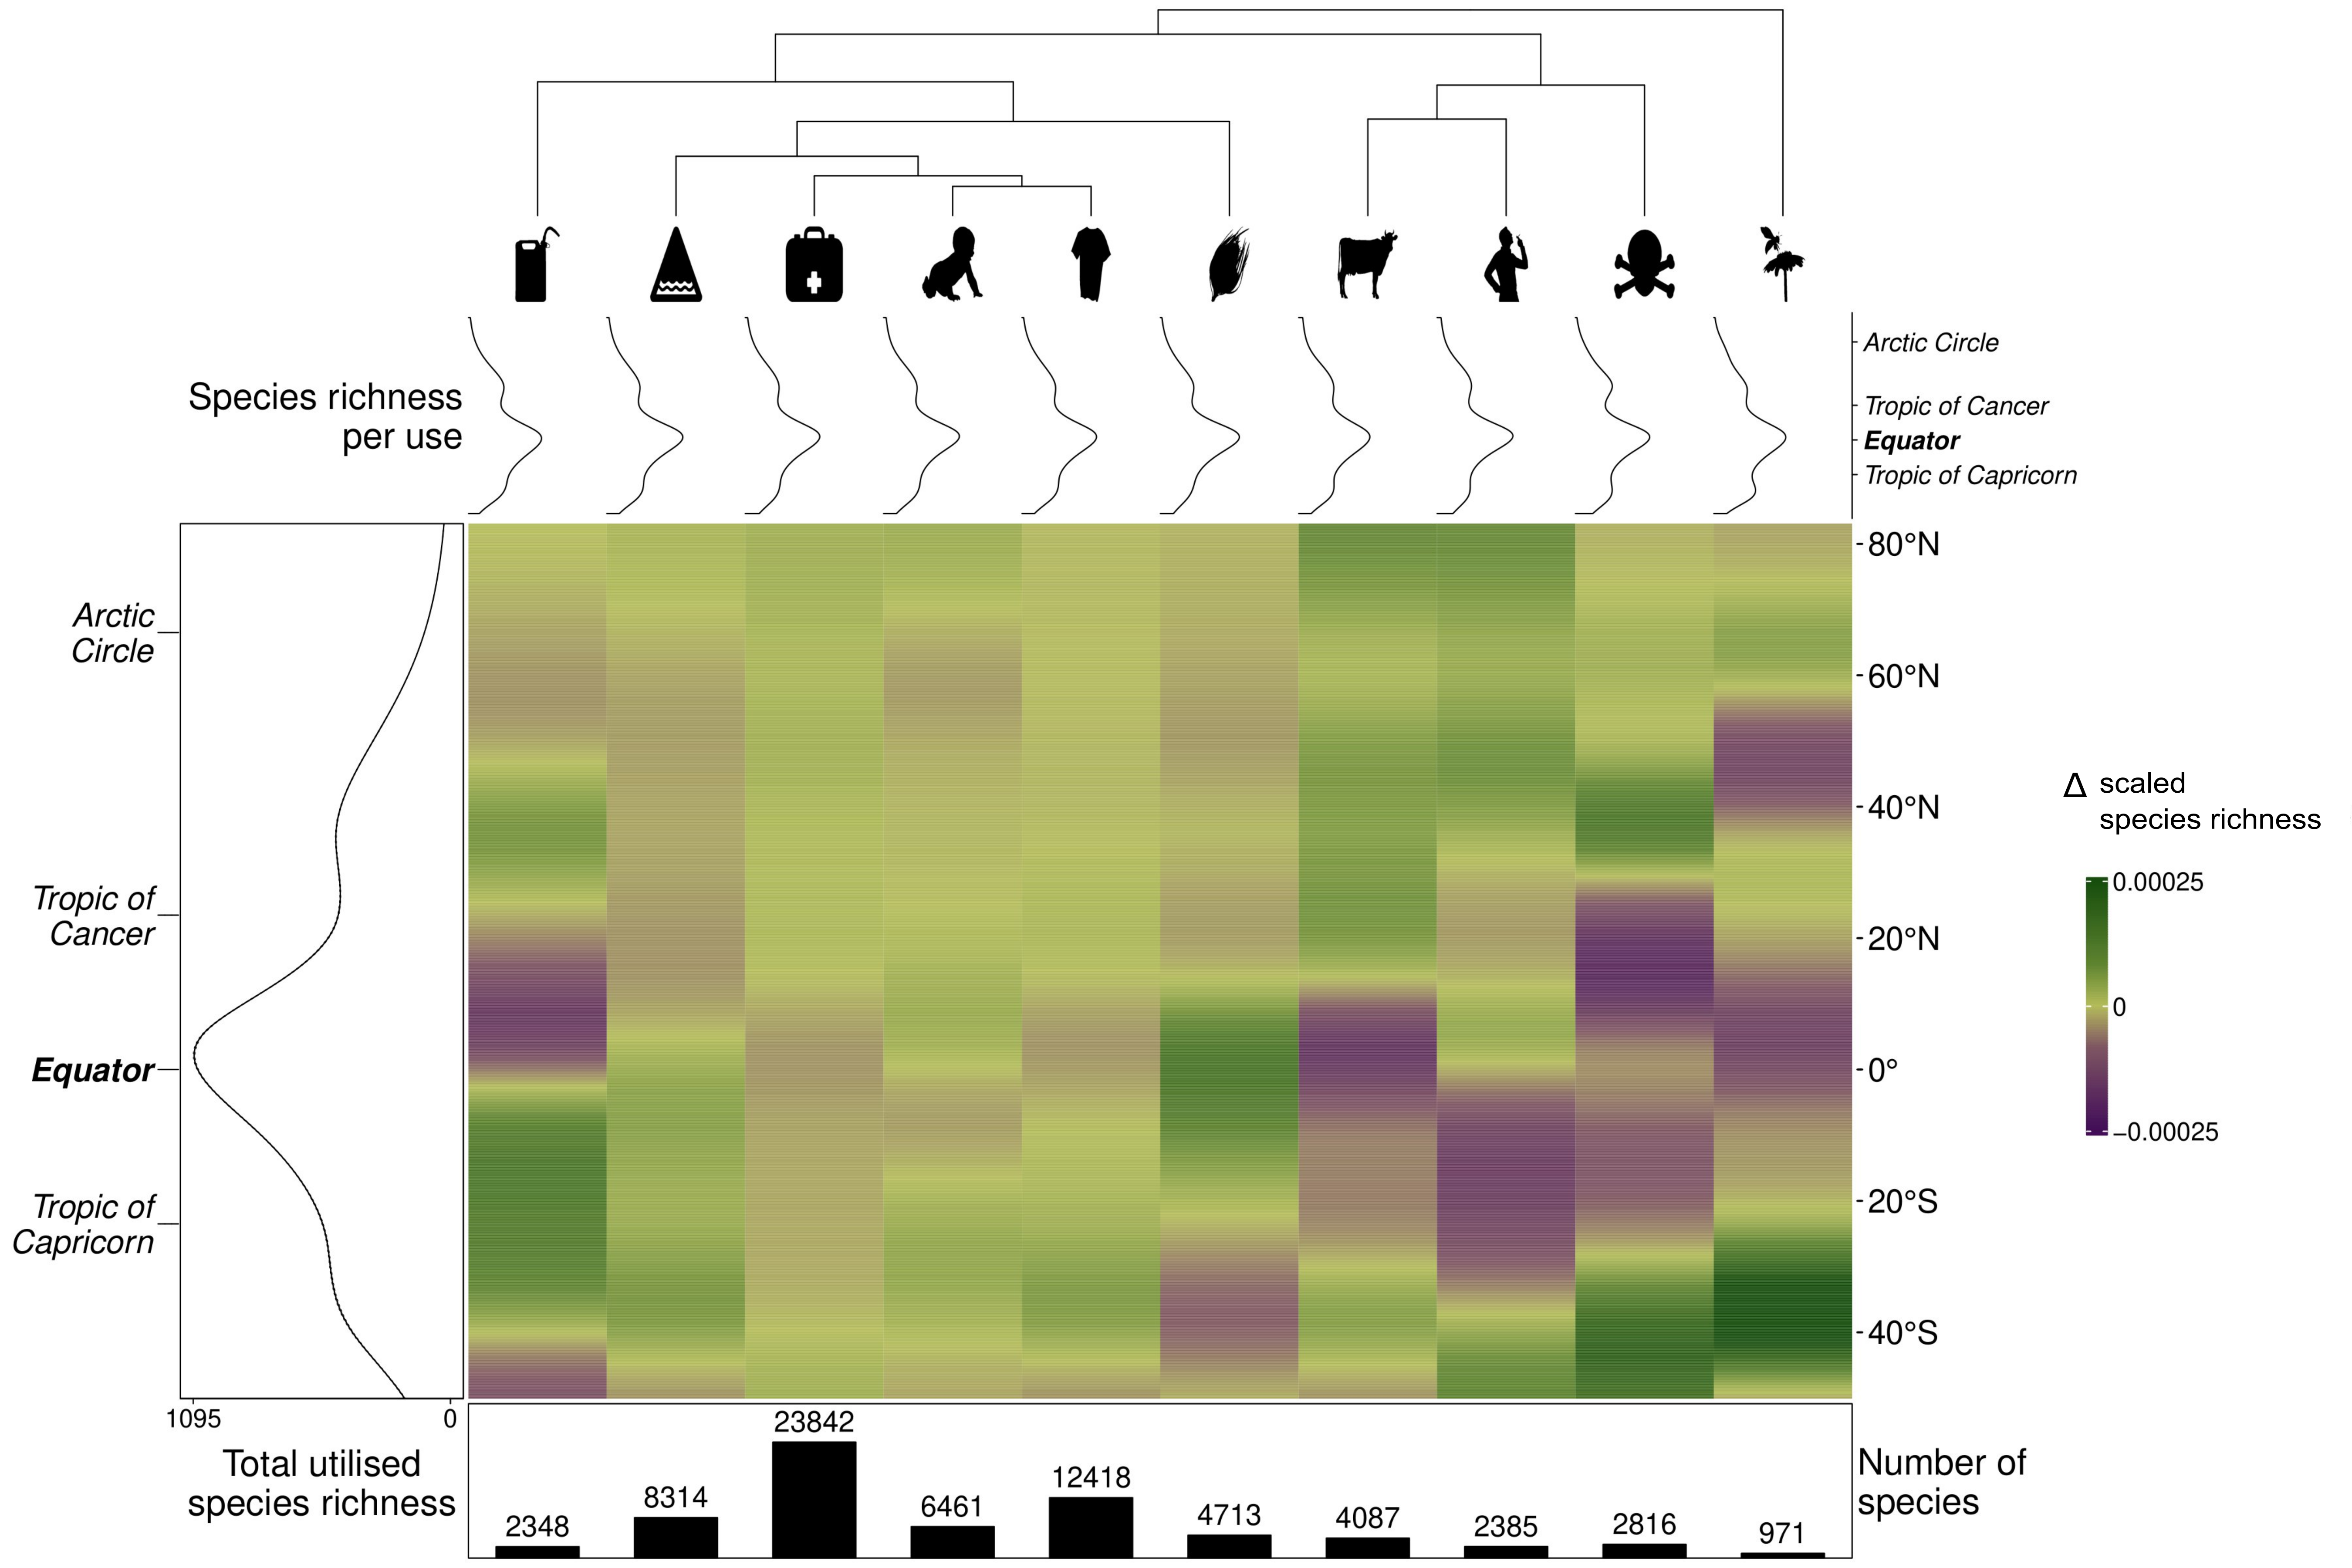
\includegraphics{heatmap_SR} \end{center}

\hypertarget{refs}{}
\begin{CSLReferences}{1}{0}
\leavevmode\vadjust pre{\hypertarget{ref-ComplexHeatmap}{}}%
Gu, Zuguang. 2022. {``Complex Heatmap Visualization.''} \emph{iMeta}.
\url{https://doi.org/10.1002/imt2.43}.

\leavevmode\vadjust pre{\hypertarget{ref-circlize}{}}%
Gu, Zuguang, Lei Gu, Roland Eils, Matthias Schlesner, and Benedikt
Brors. 2014. {``Circlize Implements and Enhances Circular Visualization
in r.''} \emph{Bioinformatics} 30: 2811--12.

\leavevmode\vadjust pre{\hypertarget{ref-terra}{}}%
Hijmans, Robert J. 2023. \emph{Terra: Spatial Data Analysis}.
\url{https://CRAN.R-project.org/package=terra}.

\leavevmode\vadjust pre{\hypertarget{ref-UsefulPlants}{}}%
Pironon S., Diazgranados M., Ondo I. 2023. {``The Global Distribution of
Plants Used by Humans.''} Journal Article.

\leavevmode\vadjust pre{\hypertarget{ref-purrr}{}}%
Wickham, Hadley, and Lionel Henry. 2023. \emph{Purrr: Functional
Programming Tools}. \url{https://CRAN.R-project.org/package=purrr}.

\leavevmode\vadjust pre{\hypertarget{ref-mgcv}{}}%
Wood, S. N. 2017. \emph{Generalized Additive Models: An Introduction
with r}. 2nd ed. Chapman; Hall/CRC.

\leavevmode\vadjust pre{\hypertarget{ref-GAMs}{}}%
Wood, S. N. 2011. {``Fast Stable Restricted Maximum Likelihood and
Marginal Likelihood Estimation of Semiparametric Generalized Linear
Models.''} \emph{Journal of the Royal Statistical Society (B)} 73 (1):
3--36.

\end{CSLReferences}

\end{document}
